%!TEX root = ../../IF.tex
%==================================================================================
\chapter{Elementos Textuais e Pós-Textuais}
%==================================================================================

Finalmente, vamos ver alguns exemplos de como lidar com figuras, tabelas, citações, códigos, algoritmos, página em modo paisagem, anexos e apêndices de acordo com as normas da ABNT, além de dicas de boas práticas de diagramacão de textos.

%==================================================================================
\section{Ilustrações}
%==================================================================================

As ilustrações, de acordo com as normas da \citeonline[seção 5.8]{NBR14724:2011}, devem atender aos seguintes requisitos: a identificação aparece na parte superior, precedida por uma palavra que a identifique (figura, desenho, esquema, etc.), seguida do número de ordem de ocorrência no texto (de forma contínua) em números arábicos, travessão e o título. Na parte inferior da ilustração, deve-se indicar a fonte consultada, mesmo sendo do próprio autor. Exemplos:

\newcommand{\proton}[1]{%
    \shade[ball color=red] (#1) circle (.25);\draw (#1) node{$+$};
}

\newcommand{\neutron}[1]{%
    \shade[ball color=green] (#1) circle (.25);
}

\newcommand{\electron}[3]{%
    \draw[rotate = #3](0,0) ellipse (#1 and #2)[color=blue];
    \shade[ball color=black] (0,#2)[rotate=#3] circle (.1);
}

\newcommand{\nucleus}{%
    \neutron{0.1,0.3}
    \proton{0,0}
    \neutron{0.3,0.2}
    \proton{-0.2,0.1}
    \neutron{-0.1,0.3}
    \proton{0.2,-0.15}
    \neutron{-0.05,-0.12}
    \proton{0.17,0.21}
}

\vspace*{10pt}
\begin{figure}[!h]
    \centering
    \caption{Legenda curta, centralizada, ocupando apenas uma linha.}
    \vspace{5pt}    
    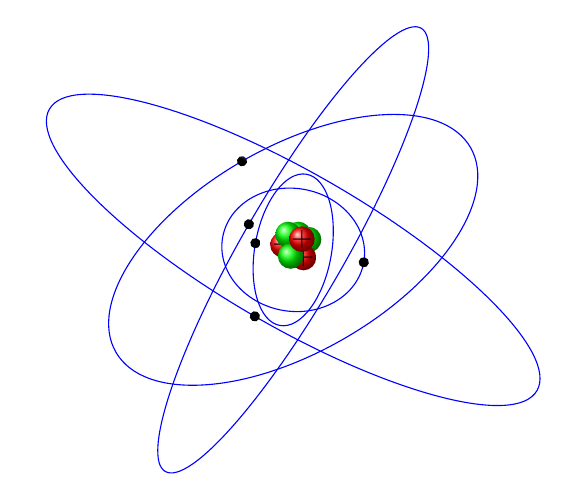
\begin{tikzpicture}[scale=0.65]
        \nucleus
        \electron{1.5}{0.75}{80}
        \electron{1.2}{1.4}{260}
        \electron{4}{2}{30}
        \electron{5}{1}{60}
        \electron{5.5}{1.5}{150}
    \end{tikzpicture}
    \vspace{5pt}    
    \fonte{adaptada de \citeonline{tikz:2015}.}
\end{figure}

\newpage

\usetikzlibrary{arrows,decorations,shapes}
\begin{figure}
\caption{Exemplo de figura com uma legenda muito grande, ocupando toda a largura da página. Neste caso, a partir da segunda linha ocorrerá identação (recuo para \mbox{a direita}).}
\vspace{5pt}
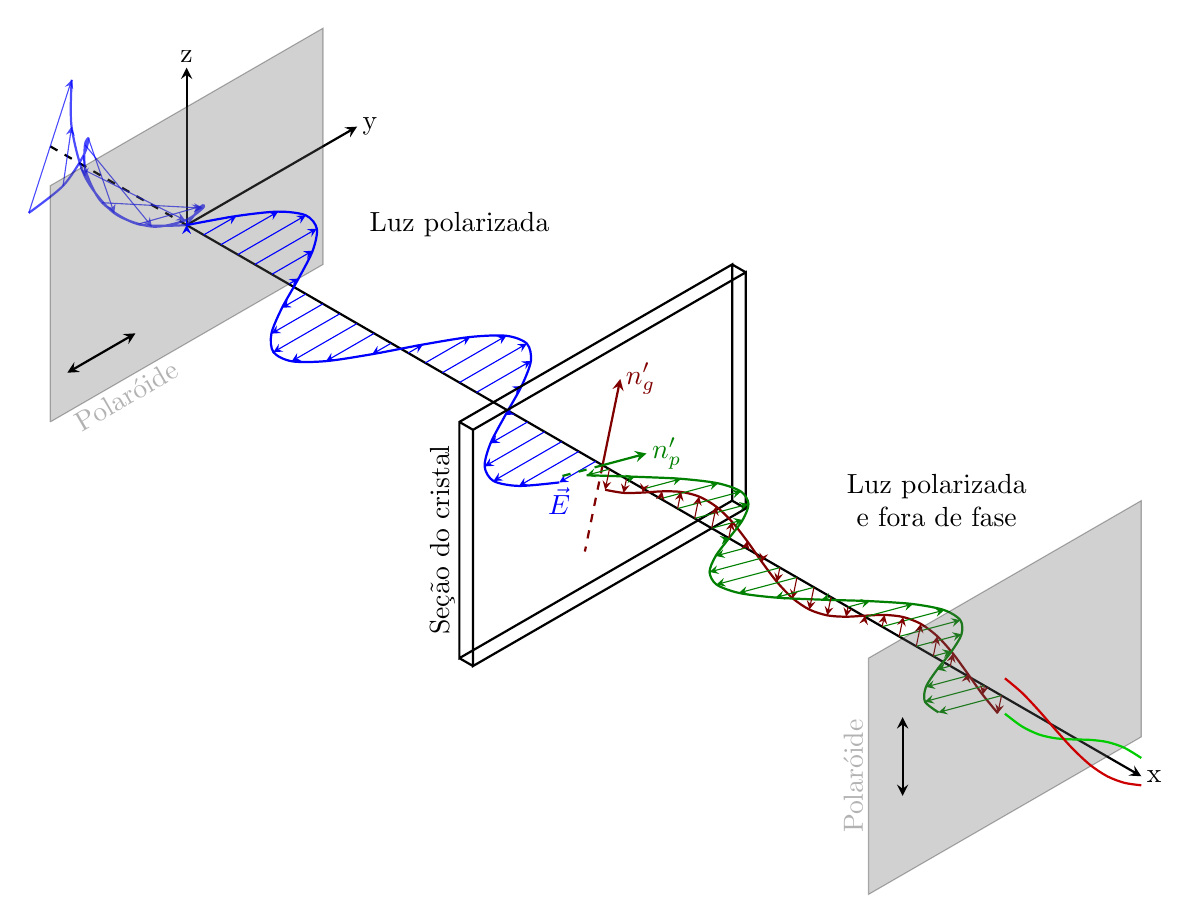
\begin{tikzpicture}[x={(0.866cm,-0.5cm)}, y={(0.866cm,0.5cm)}, z={(0cm,1cm)}, scale=1.0,
    %Option for nice arrows
    >=stealth, %
    inner sep=0pt, outer sep=2pt,%
    axis/.style={thick,->},
    wave/.style={thick,color=#1,smooth},
    polaroid/.style={fill=black!60!white, opacity=0.3},
]
    % Colors
    \colorlet{darkgreen}{green!50!black}
    \colorlet{lightgreen}{green!80!black}
    \colorlet{darkred}{red!50!black}
    \colorlet{lightred}{red!80!black}

    % Frame
    \coordinate (O) at (0, 0, 0);
    \draw[axis] (O) -- +(14, 0,   0) node [right] {x};
    \draw[axis] (O) -- +(0,  2.5, 0) node [right] {y};
    \draw[axis] (O) -- +(0,  0,   2) node [above] {z};

    \draw[thick,dashed] (-2,0,0) -- (O);

    % monochromatic incident light with electric field
    \draw[wave=blue, opacity=0.7, variable=\x, samples at={-2,-1.75,...,0}]
        plot (\x, { cos(1.0*\x r)*sin(2.0*\x r)}, { sin(1.0*\x r)*sin(2.0*\x r)})
        plot (\x, {-cos(1.0*\x r)*sin(2.0*\x r)}, {-sin(1.0*\x r)*sin(2.0*\x r)});

    \foreach \x in{-2,-1.75,...,0}{
        \draw[color=blue, opacity=0.7,->]
            (\x,0,0) -- (\x, { cos(1.0*\x r)*sin(2.0*\x r)}, { sin(1.0*\x r)*sin(2.0*\x r)})
            (\x,0,0) -- (\x, {-cos(1.0*\x r)*sin(2.0*\x r)}, {-sin(1.0*\x r)*sin(2.0*\x r)});
    }

    \filldraw[polaroid] (0,-2,-1.5) -- (0,-2,1.5) -- (0,2,1.5) -- (0,2,-1.5) -- (0,-2,-1.5)
        node[below, sloped, near end]{Polaróide};%

    %Direction of polarization
    \draw[thick,<->] (0,-1.75,-1) -- (0,-0.75,-1);

    % Electric field vectors
    \draw[wave=blue, variable=\x,samples at={0,0.25,...,6}]
        plot (\x,{sin(2*\x r)},0)node[anchor=north]{$\vec{E}$};

    %Polarized light between polaroid and thin section
    \foreach \x in{0, 0.25,...,6}
        \draw[color=blue,->] (\x,0,0) -- (\x,{sin(2*\x r)},0);

    \draw (3,1,1) node [text width=2.5cm, text centered]{Luz polarizada};

    %Crystal thin section
    \begin{scope}[thick]
        \draw (6,-2,-1.5) -- (6,-2,1.5) node [above, sloped, midway]{Seção do cristal}
                -- (6, 2, 1.5) -- (6, 2, -1.5) -- cycle % First face
            (6,  -2, -1.5) -- (6.2, -2,-1.5)
            (6,   2, -1.5) -- (6.2,  2,-1.5)
            (6,  -2,  1.5) -- (6.2, -2, 1.5)
            (6,   2,  1.5) -- (6.2,  2, 1.5)
            (6.2,-2, -1.5) -- (6.2, -2, 1.5) -- (6.2, 2, 1.5) 
                -- (6.2, 2, -1.5) -- cycle; % Second face

        %Optical indices
        \draw[darkred, ->]       (6.1, 0, 0) -- (6.1, 0.26,  0.966) node [right] {$n_{g}'$}; % index 1
        \draw[darkred, dashed]   (6.1, 0, 0) -- (6.1,-0.26, -0.966); % index 1
        \draw[darkgreen, ->]     (6.1, 0, 0) -- (6.1, 0.644,-0.173) node [right] {$n_{p}'$}; % index 2
        \draw[darkgreen, dashed] (6.1, 0, 0) -- (6.1,-0.644, 0.173); % index 2
    \end{scope}

    %Rays leaving thin section
    \draw[wave=darkred,   variable=\x, samples at={6.2,6.45,...,12}] 
        plot (\x, {0.26*0.26*sin(2*(\x-0.5) r)},  {0.966*0.26*sin(2*(\x-0.5) r)});  %n'g-oriented ray
    \draw[wave=darkgreen, variable=\x, samples at={6.2,6.45,...,12}]
        plot (\x, {0.966*0.966*sin(2*(\x-0.1) r)},{-0.26*0.966*sin(2*(\x-0.1) r)}); %n'p-oriented ray
    \draw (10,1,1) node [text width=2.5cm, text centered] {Luz polarizada e fora de fase};

    \foreach \x in{6.2,6.45,...,12} {
        \draw[color=darkgreen, ->] (\x, 0, 0) --
            (\x, {0.966*0.966*sin(2*(\x-0.1) r)}, {-0.26*0.966*sin(2*(\x-0.1) r)});
        \draw[color=darkred,   ->] (\x, 0, 0) --
            (\x, {0.26*0.26*sin(2*(\x-0.5) r)}, {0.966*0.26*sin(2*(\x-0.5) r)});
    }

    %Second polarization
    \draw[polaroid]   (12, -2,  -1.5) -- (12, -2,   1.5)  %Polarizing filter
        node [above, sloped,midway] {Polaróide} -- (12, 2, 1.5) -- (12, 2, -1.5) -- cycle;
    \draw[thick, <->] (12, -1.5,-0.5) -- (12, -1.5, 0.5); %Polarization direction

    %Light leaving the second polaroid
    \draw[wave=lightgreen,variable=\x, samples at={12, 12.25,..., 14}]
        plot (\x,{0}, {0.966*0.966*0.26*sin(2*(\x-0.5) r)}); %n'g polarized ray
    \draw[wave=lightred,  variable=\x, samples at={12, 12.25,..., 14}]
        plot (\x,{0}, {-0.26*0.966*sin(2*(\x-0.1) r)});      %n'p polarized ray

\end{tikzpicture}
\vspace{5pt}
\fonte{adaptada de \citeonline{tikz:2015}.}
\end{figure}

A classe possui mecanismos para tentar ao máximo colocar cada \emph{caption} na parte superior de objetos \emph{floats}, como figuras e tabelas.

%==================================================================================
\subsection{Código para inserir figuras em \LaTeX\ }
%==================================================================================

O formato das legendas é feito automaticamente pela classe, você deve apenas se atentar para a ordem dos comandos quando for importar uma figura. Figuras em \LaTeX\ costumam dar dor de cabeça para os iniciante, se for o seu caso, leia a documentação do pacote \citeonline{graphics:2015} para dirimir quaisquer dúvidas. A Figura \ref{texlive2014}, do Capítulo \ref{capitulo1}, foi inserida utilizando o seguinte código:

\begin{codigo}{}{Inserindo figuras em \LaTeX.}
\begin{figure}[!ht]
\centering
\caption{Faça o download do arquivo \textbf{texlive2014.iso}.}
\label{texlive2014}
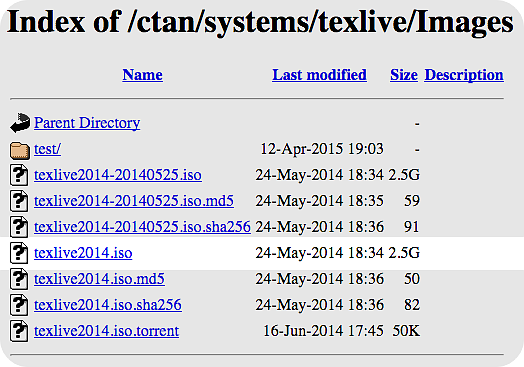
\includegraphics[width=0.7\textwidth]{./figuras/texlive2014.png}
\fonte{autor.}
\end{figure}
\end{codigo}

\noindent
note o final da instrução da linha 1, \texttt{[!h]}, ele serve para forçar com que a figura seja posicionada onde você a declarou. Mude o valor de \emph{scale} para aumentar ou diminuir a figura.

\vspace{20pt}
\noindent
\textcolor{red}{\uline{ATENÇÃO}}: o comando \Verb+\label{x}+ tem que sempre vir \textbf{depois} do comando \Verb+\caption{x}+. Regras do \LaTeX.
\vspace{10pt}

%==================================================================================
\section{Tabelas}
%==================================================================================

A ABNT recomenda seguir a formatação das tabelas do Instituto Brasileiro de Geografia e Estatística \cite{ibge:1993}. Um exemplo de tabela foi escrita no Capítulo \ref{capitulo2} (Tabela \ref{tab:opcoes_classe}). Repare na ausência das linhas verticais delimitando a tabela à esquerda e à direita. É opcional o uso de divisórias verticais no interior das tabelas para separar as colunas. O código da Tabela \ref{tab:opcoes_classe} é:


\begin{codigo}{style=lista}{Código de uma típica tabela segundo as normas da ABNT.}
\begin{table}[!h]
\centering
\caption{Opções de configuração da classe \texttt{if-ufg.cls}.}
\label{tab:opcoes_classe}
\begin{tabular}{m{4cm}m{9cm}}
\hline
\textbf{OPÇÃO} & \textbf{DESCRIÇÃO} \\ \hline
dissertacao & Dissertação de mestrado (padrão) \\ \hline
tese & Tese de doutorado \\ \hline
monografia & Monografia \\ \hline
tcc & Certificado de Especialização \\ \hline
quali-msc & Qualificação de mestrado \\ \hline
quali-doc & Qualificação de doutorado \\ \hline
frente & Modo de impressão de textos com versos brancos \\ \hline
frenteVerso & Modo de impressão de textos em frente e verso \\ \hline
abnt-alf & Usa o sistema alfabético de citação bibliográfica \\ \hline
abnt-num & Usa o sistema numérico de citação bibliográfica \\ \hline
\end{tabular}
\fonte{autor.}
\end{table}
\end{codigo}

Como pode ser observado, o estilo das legendas para as tabelas é diferente do das ilustrações. Repare também nos estilos de colunas \Verb+m{size}+ para que o conteúdo da célula fiquei alinhado verticalmente no centro.

%==================================================================================
\section{Viúvas e Órfãs}
%==================================================================================

É uma boa prática de diagramação evitar, ao máximo, o surgimento de viúvas e órfãs no texto. \textbf{Órfã} é o nome que se dá para linhas isoladas no fim de uma página e \textbf{víuva} é uma linha sozinha no início de uma página. No editorial brasileiro, o termo \emph{viúva} também é usado para as palavras que sobram sozinha na última linha de um parágrafo.

Esta classe possui mecanismos para tentar evitar o surgimento de viúvas e órfãs, mas nem sempre ela consegue controlar. Uma forma simples de contornar isto é utilizar o comando \Verb|\mbox{órfã + palavra(s) anterior(es)}| ou \Verb+\mbox{viúva}+ para forçar agrupar, porque de fato é isto que o comando \Verb+\mbox{x}+ faz, ele cria uma caixa invisível em torno dessa palavras para tentar agrupá-las, reajustando os espaços entre as palavras do parágrafo, diminuindo onde puder, para que tudo caiba naquela linha em que o comando foi invocado. 

Mas nem sempre \Verb+\mbox{x}+ fornece resultados esperados, pode ocorrer que não seja possível diminuir espaços entre as palavras do parágrafo e, então, a linha se extende para fora das margens da página. Sempre fique testando. Ou melhor, façamos um teste agora mesmo! Veja a seguir dois exemplos de uma mesma citação:

\begin{citacao}
As citações diretas, no texto, com mais de três linhas, devem ser destacadas com recuo de 4 cm da margem esquerda,
com letra menor que a do texto utilizado e sem as aspas. No caso de documentos datilografados, deve-se observar
apenas o recuo. \cite[seção 5.3]{NBR10520:2002}.
\end{citacao}

\noindent
cujo código é:

\begin{codigo}{}{Exemplo de surgimento de uma viúva.}
\begin{citacao}
As citações diretas, no texto, com mais de três linhas, devem ser destacadas com recuo de 4 cm da margem esquerda,
com letra menor que a do texto utilizado e sem as aspas. No caso de documentos datilografados, deve-se observar
apenas o recuo. \cite[seção 5.3]{NBR10520:2002}.
\end{citacao}
\end{codigo}

\noindent
Contudo, usando o \Verb+\mbox{x}+ pode-se evitar esta viúva:

\begin{citacao}
As citações diretas, no texto, com mais de três linhas, devem ser destacadas com recuo de 4 cm da margem esquerda,
com letra menor que a do texto utilizado e sem as aspas. No caso de documentos datilografados, deve-se observar
apenas o recuo. \mbox{\cite[seção 5.3]{NBR10520:2002}.}
\end{citacao}

\noindent
\\

\begin{codigo}{}{Exemplo de remoção de viúva com o uso do \textbackslash{mbox\{x\}}.}
\begin{citacao}
As citações diretas, no texto, com mais de três linhas, devem ser destacadas com recuo de 4 cm da margem esquerda,
com letra menor que a do texto utilizado e sem as aspas. No caso de documentos datilografados, deve-se observar
apenas o recuo. \mbox{\cite[seção 5.3]{NBR10520:2002}.}
\end{citacao}
\end{codigo}

\noindent
Observe como os espaços entre as palavras do parágrafo foram reajustados.

%==================================================================================
\section{Códigos de Programas}
%==================================================================================

%==================================================================================
\subsection{Código fonte}
%==================================================================================

Para imprimir códigos de programas de uma maneira mais agradável, esta classe utiliza as facilidades do pacote \citeonline{listings:2015}. Nas páginas anteriores, você observou vários exemplos do uso do ambiente \Verb+\begin{codigo}{language=x}{x}...\end{codigo}+ para mostrar algumas linhas de códigos. Esta classe implementa um estilo próprio chamado \texttt{codeStyle}. Se a linguagem que você importar não estiver sendo interpretada corretamente, por exemplo, faltando destacar algumas palavras internas da linguagem como um \emph{if...else}, leia a documentação do pacote. 

\vspace{20pt}
\noindent
\textcolor{red}{\uline{ATENÇÃO}}: não altere o estilo da classe, crie o seu próprio estilo para atender a sua linguagem! Deixe a classe sem alterações para evitar problemas de atualizações futuras.
\vspace{20pt}

Caso for alterar o estilo, basta definir um estilo próprio:

\begin{center}
\colorbox{black!8}{\ttfamily\rlap{\textbackslash{lstdefinestyle\{<nome\_do\_estilo>\}\{<parâmetros>\}}}\hspace{\linewidth}\hspace{-2\fboxsep}}
\end{center}

\noindent
e depois informar no ambiente: 

\begin{codigo}{style=lista,escapechar=+}{Usando o seu próprio estilo no ambiente de códigos.}
+\verb!\begin{codigo}{style=<nome_do_estilo>,language=<linguagem>}{<legenda>}!+
.
.
.
+\verb!\end{codigo}!+
\end{codigo}

%==================================================================================
\subsection{Importando um código fonte}
%==================================================================================

É possível também importar diretamente um código fonte presente em um diretório com o comando:

\begin{center}
\colorbox{black!8}{\ttfamily\rlap{\textbackslash{importarcodigo\{language=<linguagem>\}\{<legenda>\}\{\emph{<./path/to/program>}\}}}\hspace{\linewidth}\hspace{-2\fboxsep}}
\end{center}

\begin{codigo}{language=C}{Código digitado dentro do ambiente de \textit{codigo}.}
void insertionSort( int* v, int n )
{
  int i   = 0;
  int j   = 1;
  int aux = 0;
  
  while (j < n)
  {
    aux = v[j];
    i   = j - 1;
    while ((i >= 0) && (v[i] > aux))
    {
      v[i + 1] = v[i];
      i = i - 1;
    }
    v[i + 1] = aux;
    j = j + 1;
  }
}
\end{codigo}

\importarcodigo{language=C}{Código importado de ./programas/insertionsort.c}{./programas/insertionsort.c}

O pacote \citeonline{listings:2015} é extremamente poderoso, existem inúmeras variedades de opções. É possível, por exemplo, escolher quais as linhas do código que devem ser exibidas, caso não queira imprimir todo o código fonte. Basta usar as opções \Verb+firstline=<número>+ e \Verb+lastline=<número>+ para selecionar o intervalo desejado. Por exemplo, no caso do código anterior, para imprimir apenas da linha 7 à linha 18, englobando a estrutura do \Verb+while{...}+:

\begin{codigo}{language=C}{Selecionando um intervalo de código para imprimir.}
\importarcodigo{language=C,firstline=7,lastline=18}{Código importado de ./programas/insertionsort.c}{./programas/insertionsort.c}
\end{codigo}

\noindent
o resultado é:

\importarcodigo{label={codigo:importcodebiglegend},language=C,firstline=7,lastline=18}{Intervalo de código importado de ./programas/insertionsort.c com uma legenda muito grande.}{./programas/insertionsort.c}

%==================================================================================
\subsection{Referência \texttt{\textbackslash{ref\{x\}}} a um código fonte}
%==================================================================================

Para fazer referência a algum código ao longo do texto com o comando \Verb+\ref{x}+, o \Verb+\label{x}+ é declarado de uma forma diferente do que a explicada para as ilustrações. O pacote \texttt{listings} prefere que seja declarado da seguinte forma:

\begin{center}
\colorbox{black!8}{\ttfamily\rlap{\textbackslash{begin\{codigo\}\{label={<nome>},(...)\}}...\textbackslash{end\{codigo\}}}\hspace{\linewidth}\hspace{-2\fboxsep}}
\end{center}

\noindent
Posso agora, por exemplo, fazer uma referência ao Código \ref{codigo:importcodebiglegend} da seguinte maneira:

\begin{codigo}{language=C}{Exemplo de como fazer referência a um código no texto.}
\importarcodigo{label={codigo:importcodebiglegend},language=C,firstline=7,lastline=18}{Intervalo de código importado de ./programas/insertionsort.c com uma legenda muito grande.}{./programas/insertionsort.c}
\end{codigo}

\noindent
e depois usando o comando \Verb+\ref{codigo:importcodebiglegend}+.

%==================================================================================
\subsection{Algoritmos}
%==================================================================================

É utilizado o ambiente \Verb+\begin{algoritmo}...\end{algoritmo}+, baseado no pacote \citeonline{algorithm2e:2015}, para escrever algoritmos ou pseudo-códigos. Por exemplo:

\begin{algoritmo}
\caption{$MSR(A,i,j)$.}\label{alg:algoritmo}
 \DontPrintSemicolon
 \LinesNumbered
 \SetAlgoLined
 \BlankLine
 \Entrada{vetor $A[i\,.\,.\,j]$, inteiros não negativos $i$ e $j$.}
 \Saida{vetor $A[i\,.\,.\,j]$ ordenado.}
 \BlankLine
 $n \leftarrow j - i$.\;
 \eSe{$(n<4)$}
   {Ordene com $\leq 3$ comparações.}
   {Divida $A$ em $\lceil\sqrt{n}\,\,\rceil$ subvetores de comprimento máximo $\lfloor\sqrt{n}\,\rfloor$.\;
    Aplique $MSR$ a cada um dos subvetores.\;
    Intercale os subvetores.\;}    
\end{algoritmo}

\noindent
cujo código é:

\begin{codigo}{style=lista}{Exemplo de uso do ambiente \textit{algoritmo}.}
\begin{algoritmo}
\caption{$MSR(A,i,j)$.}\label{alg:algoritmo}
 \DontPrintSemicolon
 \LinesNumbered
 \SetAlgoLined
 \BlankLine
 \Entrada{vetor $A[i\,.\,.\,j]$, inteiros não negativos $i$ e $j$.}
 \Saida{vetor $A[i\,.\,.\,j]$ ordenado.}
 \BlankLine
 $n \leftarrow j - i$.\;
 \eSe{$(n<4)$}
   {Ordene com $\leq 3$ comparações.}
   {Divida $A$ em $\lceil\sqrt{n}\,\,\rceil$ subvetores de comprimento máximo $\lfloor\sqrt{n}\,\rfloor$.\;
    Aplique $MSR$ a cada um dos subvetores.\;
    Intercale os subvetores.\;}
\end{algoritmo}
\end{codigo}

Repare que neste caso o uso de \Verb+\caption{x}+ e \Verb+\label{x}+ é feito da mesma maneira como nas ilustrações e tabelas e, portanto, pode-se fazer uma referência ao Algoritmo \ref{alg:algoritmo} da maneira usual.

%==================================================================================
\section{Modo Paisagem}
%==================================================================================

A seguir, um exemplo de como usar o ambiente \emph{paisagem}.

\begin{paisagem}
O ambiente \Verb+\begin{paisagem}...\end{paisagem}+ foi criado baseado no pacote \texttt{lscape}. É útil, por exemplo, quando se deseja imprimir algo que não cabe no modo ``retrato'', como tabelas com grande número de colunas. Seu uso é bem fácil:

\begin{codigo}{style=lista}{Exemplo de uso do ambiente \textit{paisagem}.}
\begin{paisagem}
.
.
.
\end{paisagem}
\end{codigo}
\end{paisagem}

%==================================================================================
\section{Citações}
%==================================================================================

As normas da ABNT NBR 6023:2002 e NBR 10520:2002 determinam o modo de se fazer citações bibliográficas. Esta classe faz uso do pacote \citeonline{abntex2cite:2015}, que implementa as vastas regrinhas das normas de citação da ABNT. É extremamente recomendável consultar a documentação do pacote.

Normalmente, os comandos mais utilizados são:

\begin{itemize}
\item  \Verb+\cite[x]{bibkey}+: usado quando o \emph{sobrenome} do autor ou nome da instituição é citado em letras maiúsculas e ano separado por vírgula, tudo entre parênteses. Exemplos:

\begin{itemize}
\item \Verb+\cite{NBR10520:2002}+: \cite{NBR10520:2002};
\item \Verb+\cite[p. 2]{NBR10520:2002}+: \cite[p. 2]{NBR10520:2002}.
\end{itemize}

\item  \Verb+\citeonline[x]{bibkey}+: usado quando o \emph{sobrenome} do autor ou nome da instituição é indicado com apenas a primeira letra em maiúsculo, seguido do ano entre parênteses. Uma excessão é quando o nome da instituição é dado por uma sigla, em que esta é representada em letras maiúsculas. Exemplos: 

\begin{itemize}
\item \Verb+\citeonline{texlive:2015}+: \citeonline{texlive:2015};
\item \Verb+\citeonline[p. 2]{NBR10520:2002}+: \citeonline[p. 2]{NBR10520:2002}.
\end{itemize}

\end{itemize}

Como você deve ter percebido, caso seja necessário indicar a página, capítulo ou volume da fonte consultada, deve ser usado o primeiro campo de ambos os comandos. Vejas outros exemplos a seguir.

%==================================================================================
\subsection{Citação Indireta}
%==================================================================================

Nas citações indiretas não ocorre a transcrição textual de parte da obra do autor ou instituição, servem como modo de referência complementar para o contexto do parágrafo \cite{NBR10520:2002}. É opcional citar indicações de páginas ou seções de consulta, como pode ser visto em \citeonline[p. 2]{NBR10520:2002}. 

%==================================================================================
\subsection{Citação Direta}
%==================================================================================
\label{citacaodireta}
Consiste na transcrição textual de parte da obra do autor ou instituição. Segundo \citeonline[p. 2]{NBR10520:2002}, ``as citações diretas, no texto, de até três linhas, devem estar contidas entre aspas duplas. As aspas simples são utilizadas para indicar citação no interior da citação''. 

Para citações acima de três linhas, de acordo com a ABNT:

\begin{citacao}
As citações diretas, no texto, com mais de três linhas, devem ser destacadas com recuo de 4 cm da margem esquerda,
com letra menor que a do texto utilizado e sem as aspas. No caso de documentos datilografados, deve-se observar
apenas o recuo. \mbox{\cite[p. 2]{NBR10520:2002}.}
\end{citacao}

\noindent
Para atender à esta norma, foi criado o ambiente \emph{citacao}, cujo código é:

\begin{codigo}{style=lista,label={codigo:citacaolonga}}{Uso do ambiente \textbackslash{begin\{citacao\}}...\textbackslash{end\{citacao\}}.}
\begin{citacao}
As citações diretas, no texto, com mais de três linhas, devem ser destacadas com recuo de 4 cm da margem esquerda,
com letra menor que a do texto utilizado e sem as aspas. No caso de documentos datilografados, deve-se observar
apenas o recuo. \mbox{\cite[seção 5.3]{NBR10520:2002}.}
\end{citacao}
\end{codigo}
\label{citacao}

%==================================================================================
\section{Referências Bibliográficas}
%==================================================================================
\label{refbibliografica}
Existem dois modos de referências bibliográficas: (1) sistema numérico (2) sistema alfabético. Sim! A \citeonline{NBR6023:2000} autoriza o uso do sistema numérico para as referências bibliográficas. Para informar o estilo que deseja em seu trabalho acadêmico, escolha entre \textbf{abnt-alf} ou \textbf{abnt-num} nas opções de \Verb+\documentclass[opções]{if-ufg}+. 

No sistema numérico, muito utilizado pelas faculdades da área de exatas, a referência aparece como um número entre colchetes (ex.: [1]), neste caso, utilize o comando \Verb+\cite[x]{bibkey}+. Portanto, atente-se para o uso do comando \Verb+\citeonline[x]{bibkey}+, pois a referência numérica irá aparecer \emph{sem os colchetes}, mostrando apenas o número, podendo causar confusão em algumas circunstâncias.

Ainda, com o uso do pacote \emph{backref} é possível saber onde exatamente uma determinada referência foi citada, ou quantas vezes ela foi citada, com a mensagem: ``Citado na página <pag>.'' ou ``Citado <x> vezes nas páginas <pags>.''.

\vspace{20pt}
\noindent
\textcolor{red}{\uline{ATENÇÃO}}: orientadores e membros de banca, este é um recurso excelente para verificar se as citações foram feitas corretamente e onde elas aparecem ao longo do texto, facilitando a avaliação da revisão bibliográfica.
\vspace{10pt}

É extremamente recomendável utilizar um arquivo \emph{.bib} com as referências bibliográficas e, depois, no arquivo \texttt{pos\_config.tex} importar com o comando: 

\begin{center}
\colorbox{black!8}{\ttfamily\rlap{\textbackslash{bibliography\{./pos\_textuais/bibliografia/bibliografia\}}}\hspace{\linewidth}\hspace{-2\fboxsep}}
\end{center}
 
Existem bons gerenciadores de referências bibliográficas, com ótimos recursos, tais como o \citeonline{jabref:2015} para Windows, Linux e Mac OS X, porém, para o Mac OS X, indico e utilizo o \citeonline{bibdesk:2015}.

%==================================================================================
\section{Apêndices}
%==================================================================================

Segundo a \citeonline[p. 2]{NBR14724:2011}, o \textbf{apêndice} é um ``texto ou documento \emph{elaborado} pelo autor, a fim de complementar sua argumentação, sem prejuízo da unidade nuclear do trabalho''. 

Foi criado o ambiente \Verb+\begin{apendices}...\end{apendices}+ para incluir os capítulos que farão parte dos apêndices, utilizando da seguinte forma:

\begin{codigo}{}{Exemplo de uso do ambiente \emph{apendices}.}
\begin{apendices}

\chapter{Apêndice 1}
....
\chapter{Apêndice 2}
...

\end{apendices}
\end{codigo}

No caso dos apêndices, para as ``numerações'' dos capítulos são usadas as letras do alfabeto em maiúsculo, como por exemplo: \emph{Apêndice A, Apêndice B,} etc.

%==================================================================================
\section{Anexos}
%==================================================================================
Um \textbf{anexo} consiste de um ``texto ou documento \emph{não elaborado} pelo autor, que serve de fundamentação, comprovação e ilustração'' \cite[p. 2]{NBR14724:2011}.

A classe implementa o ambiente \Verb+\begin{anexos}...\end{anexos}+, com um modo de uso idêntico como o feito para os apêndices, porém os anexos são ordenados numericamente, ou seja, \emph{Anexo 1, Anexo 2,} etc.

\vspace{20pt}
\noindent
\textcolor{red}{\uline{ATENÇÃO}}: note que tanto os apêndices quanto os anexos fazem parte dos elementos pós-textuais, portanto, mantenha sempre atualizado o arquivo \texttt{pos\_config.tex}.

%==================================================================================
\section{Considerações Finais}
%==================================================================================

A classe \texttt{if-ufg.cls} foi concebida para tentar atender a todos os tipos de trabalhos acadêmicos. Caso você não for utilizar certos recursos, como por exemplo a ficha catalográfica (CDU) para um trabalho de qualificação, apenas comente a linha no arquivo \emph{pre\_config.tex}. Se o seu trabalho não contiver códigos ou algoritmos, comente os comandos \Verb+\listadealgoritmos+ e \Verb+\listadecodigos+, e assim por diante. Então bons estudos, bom trabalho e divirta-se! =)